\chapter{Исследовательская часть}

В данном разделе будет проведен анализ зависимости количества строк на время выполнения хранимой процедуры в базе данных.

\section{Технические характеристики}

Технические характеристики устройства, использовавшегося для выполнения замеров, представлены ниже.

\begin{itemize}[label=---]
	\item Процессор: AMD Ryzen 7--5800H with Radeon Graphics~\cite{amd_ryzen}.
	\item Оперативная память: 16 ГБайт.
	\item Операционная система: Windows 11 Home~\cite{windows}.
\end{itemize}

При замерах времени ноутбук был включен в сеть электропитания и был нагружен только системными приложениями.

\section{Сравнительный анализ работы со \newline строками в хранимой процедуре}

Время выполнения процедуры представляет собой критический параметр, определяющий производительность базы данных.
Более длительное время выполнения может привести к замедлению работы приложения и негативному влиянию на пользовательский опыт~\cite{microsoft}.

В процессе написания курсового проекта была найдена связь между количеством строк, обрабатываемых хранимой процедурой, и временем ее выполнения при работе со строками.
Для потверждения этой гипотезы был проведен сравнительный анализ работы с разным количеством строк.
В качестве хранимой процедуры была выбрана процедура, возвращающая вероятность задержки рейса.


Замеры производились на следующих параметрах:
\begin{enumerate}
	\item количество строк, обрабатываемых хранимой процедурой;
	\item время выполнения --- рассчитывается как среднее значение из 10 измерений.
\end{enumerate}

На рисунке~\ref{fig:myplot} представлен график зависимости времени выполнения хранимой процедуры от количества строк.

\begin{figure}[H]
	\centering
	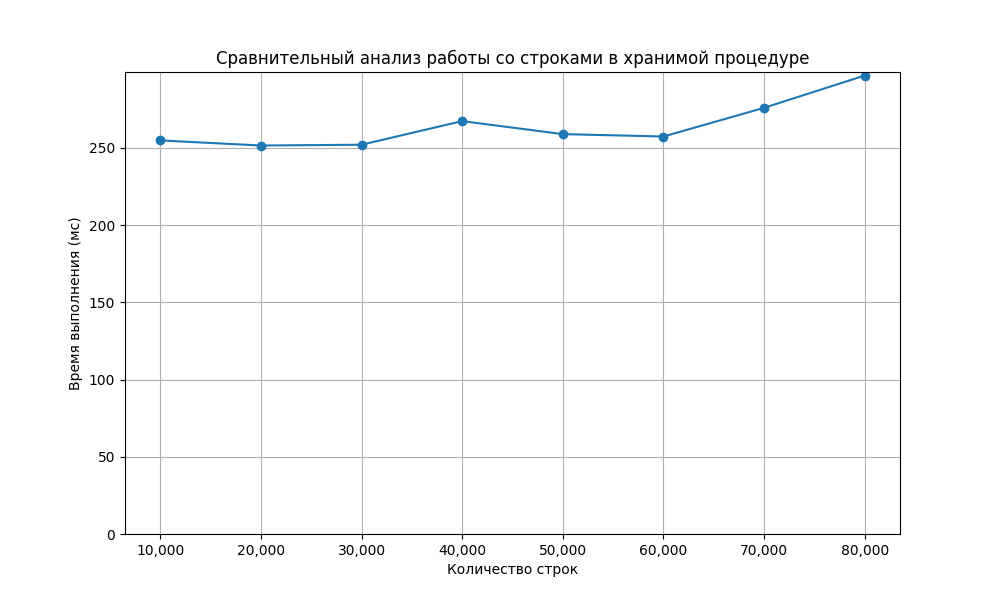
\includegraphics[scale=0.4]{inc/myplot}
	\caption{График сравнительного анализа работы со строками в хранимой процедуре}
	\label{fig:myplot}
\end{figure}

\section*{Выводы}
\addcontentsline{toc}{section}{Выводы}
В данном разделе был проведен сравнительный анализ работы с разным количеством строк в хранимой процедуре.
По результатам анализа было установлено, что время выполнения хранимой процедуры зависит от количества обрабатываемых строк --- с увеличением количества строк время выполнения хранимой процедуры линейно увеличивается.
Результаты анализа позволяют сделать выводы о том, что для оптимизации работы с базой данных необходимо уменьшать количество строк, обрабатываемых хранимой процедурой.



